\section{Diagnóstico de cáncer de mamas}

%%--------------------------------------------------------------------------------------------------------------------------------------------------

\subsection{Introducción}

%%--------------------------------------------------------------------------------------------------------------------------------------------------

\subsection{Modelo}

La red elegida está compuesta por la capa de entrada con 10 neuronas (una por cada feature), una capa oculta con 12 neuronas y la capa de salida con una sola neurona. 

%%--------------------------------------------------------------------------------------------------------------------------------------------------

\subsection{Implementación}

%%--------------------------------------------------------------------------------------------------------------------------------------------------

\subsubsection{Prepocesamiento de datos}

Se normalizan los ejemplos del dataset.

%%--------------------------------------------------------------------------------------------------------------------------------------------------

\subsubsection{Pseudocódigo}

%%--------------------------------------------------------------------------------------------------------------------------------------------------

\subsection{Ejecución}

%%--------------------------------------------------------------------------------------------------------------------------------------------------

\subsubsection{Modo de uso}

Para entrenar la red:

Ejemplo: 

\noindent\texttt{python trainnet1.py -m TP1/models/ej1.lmodel -o ./salida.params -t 900 -e 0.05 -l 0.005 -b 1 -x TP1/ds/tp1\_ej1\_training.csv}

Explicación:

\begin{tabular}{ l l }
-m & Ruta al archivo de modelo (lmodel) \\
-o & Ruta del archivo de salida con los pesos\\
-t & Epochs\\
-e & Epsilon\\
-l & Learning rate\\
-b & Size minibatch (default 1)\\
-x & Archivo de samples\\
\end{tabular}

\begin{tabular}{ c l }
-m M & Ruta al archivo de modelo (lmodel)\\
-p  O & Ruta del archivo de entrada con los pesos\\
-x  X & Archivo de features\\
\end{tabular}

Para predecir:

Ejemplo:

\noindent\texttt{\small{python predict1.py -m TP1/models/ej1.lmodel -p TP1/salida.params -x TP1/ds/tp1\_ej1\_training.csv}}

Explicación:

\begin{tabular}{ l l }
-m & Ruta al archivo de modelo (lmodel)\\
-p & Ruta del archivo de entrada con los pesos\\
-x & Archivo de features\\
\end{tabular}

%%--------------------------------------------------------------------------------------------------------------------------------------------------

\subsubsection{Requerimientos}

%%--------------------------------------------------------------------------------------------------------------------------------------------------

\subsection{Resultados}

%%--------------------------------------------------------------------------------------------------------------------------------------------------

\subsubsection{Pruebas con distintos learning rates}

Parámetros elegidos fijos:

\begin{itemize}
\item beta = 5
\item mini\_batch\_size = 1
\item epochs = 1000
\item epsilon = 0.05
\item reg\_param = 0.0
\end{itemize}


\begin{figure}[h]	
	\begin{subfigure}[b]{0.5\textwidth}
		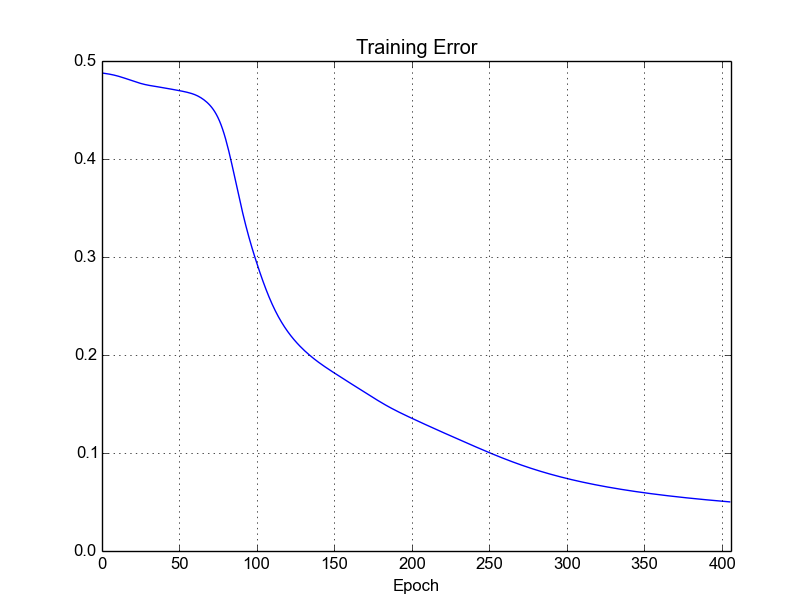
\includegraphics[width=\linewidth]{fig/trainingerror_lr0,0075_eps0,05_regparam0,00_beta5_batch1.png}
	\end{subfigure}
	\begin{subfigure}[b]{0.5\textwidth}
		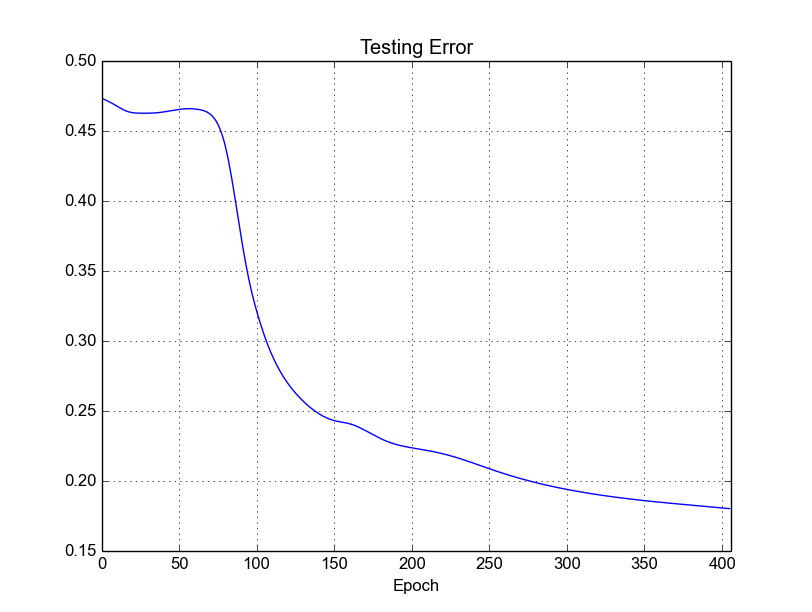
\includegraphics[width=\linewidth]{fig/valerror_lr0,0075_eps0,05_regparam0,00_beta5_batch1.png}
	\end{subfigure}

	\caption{\textbf{learning rate: 0.0075}}
\end{figure}


\begin{figure}[h]	
	\begin{subfigure}[b]{0.5\textwidth}
		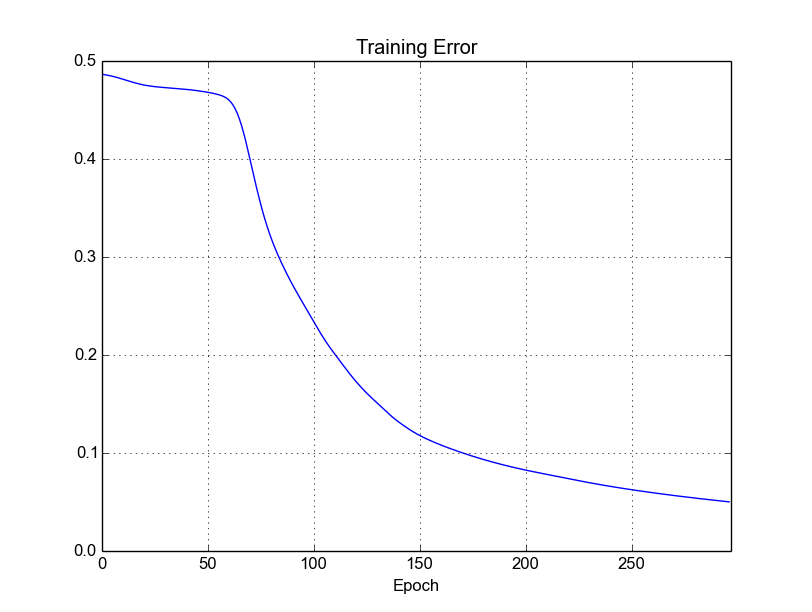
\includegraphics[width=\linewidth]{fig/trainingerror_lr0,01_eps0,05_regparam0,00_beta5_batch1.png}
	\end{subfigure}
	\begin{subfigure}[b]{0.5\textwidth}
		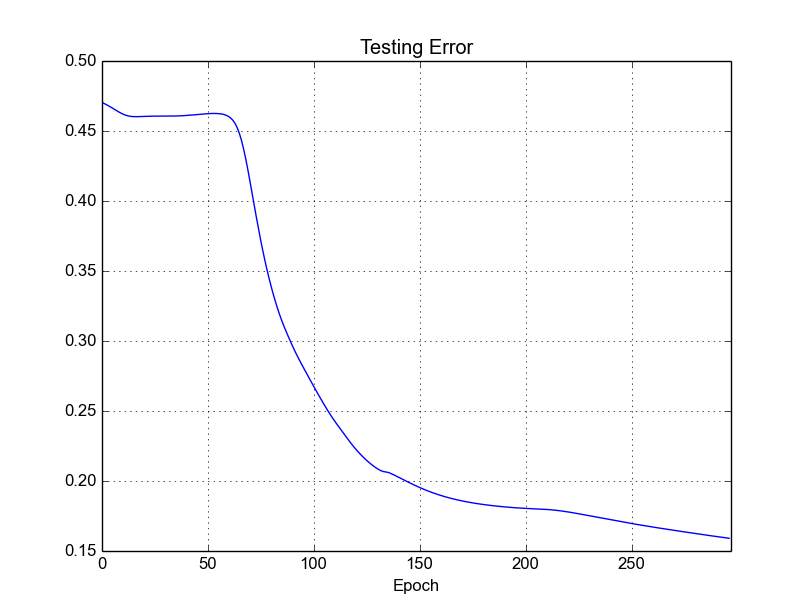
\includegraphics[width=\linewidth]{fig/valerror_lr0,01_eps0,05_regparam0,00_beta5_batch1.png}
	\end{subfigure}

	\caption{\textbf{learning rate: 0.01}}
\end{figure}

En estos gráficos se puede ver que el error fue menor a epsilon = 0,05.
 En el primero de ellos el coeficiente de aprendizaje utilizado es 
 0.0075 y en el segundo 0.01. Se observa que coeficiente de aprendizaje
  más pequeño el error sube. Por otro lado, se puede ver que cuanto 
  más chico paso más épocas fueron necesarias para minimizar el error. 
Por lo que elegimos 0.01 como mejor learning rate.

\newpage

\begin{figure}[h]	
	\begin{subfigure}[b]{0.5\textwidth}
		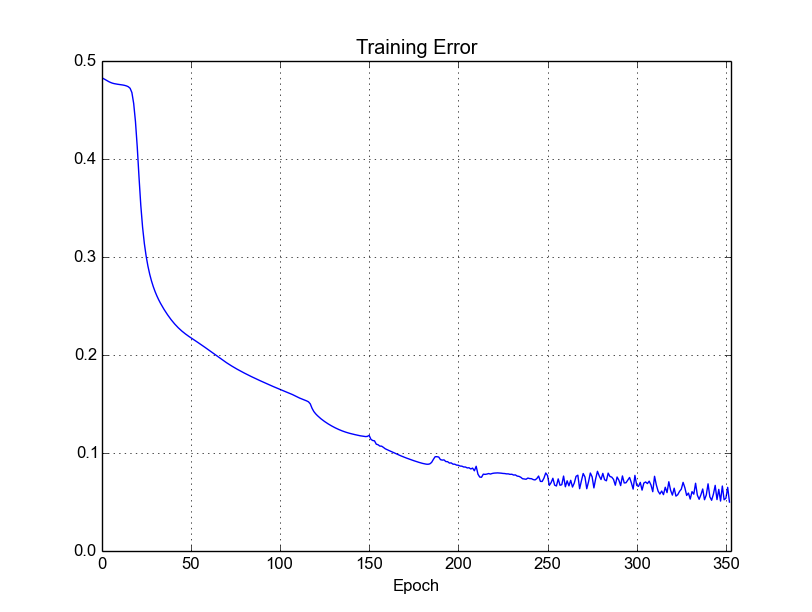
\includegraphics[width=\linewidth]{fig/trainingerror_lr0,025_eps0,05_regparam0,00_beta5_batch1.png}
	\end{subfigure}
	\begin{subfigure}[b]{0.5\textwidth}
		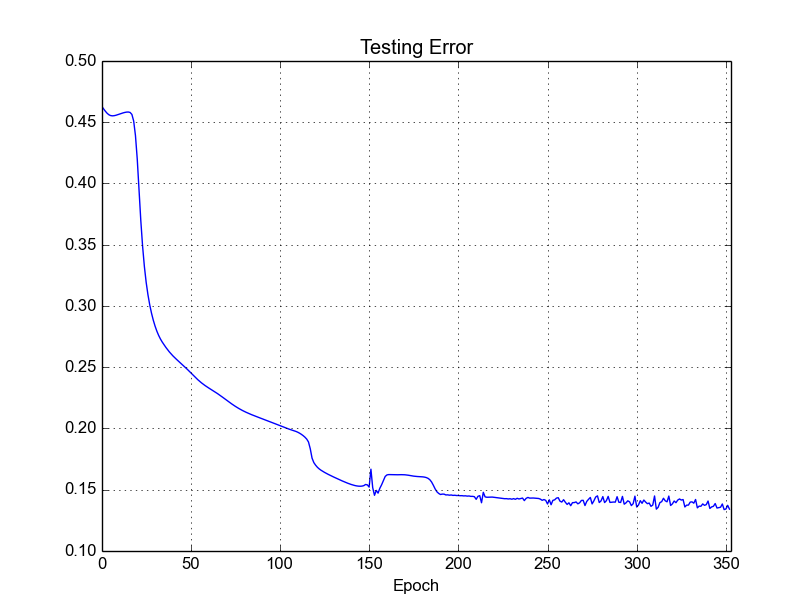
\includegraphics[width=\linewidth]{fig/valerror_lr0,025_eps0,05_regparam0,00_beta5_batch1.png}
	\end{subfigure}

	\caption{\textbf{learning rate: 0.025}}
\end{figure}

\begin{figure}[h]	
	\begin{subfigure}[b]{0.5\textwidth}
		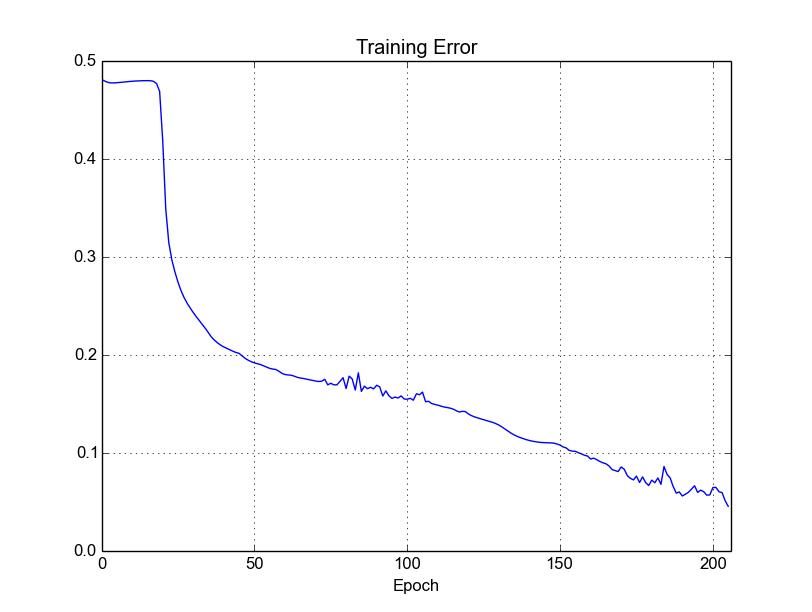
\includegraphics[width=\linewidth]{fig/trainingerror_lr0,05_eps0,05_regparam0,00_beta5_batch1.png}
	\end{subfigure}
	\begin{subfigure}[b]{0.5\textwidth}
		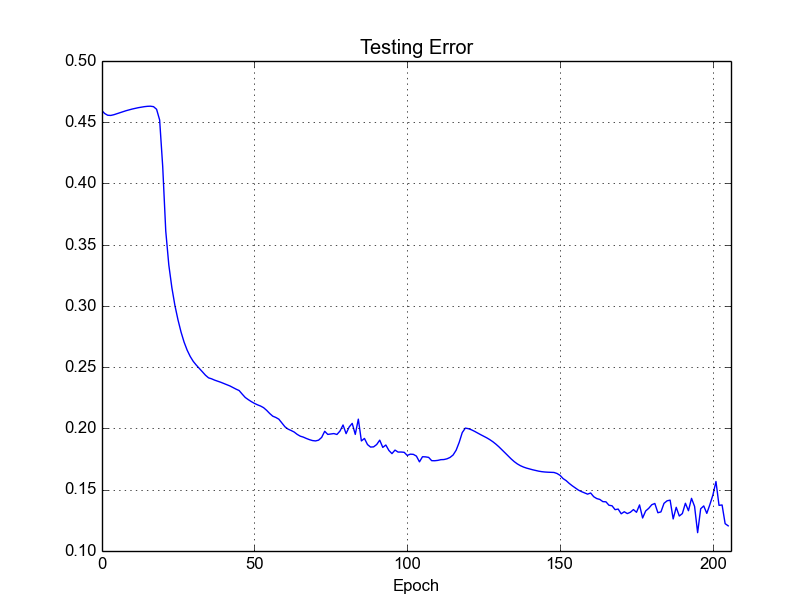
\includegraphics[width=\linewidth]{fig/valerror_lr0,05_eps0,05_regparam0,00_beta5_batch1.png}
	\end{subfigure}

	\caption{\textbf{learning rate: 0.05}}
\end{figure}

Estos dos gráficos muestran que al ser el coeficiente de aprendizaje es muy grande y se han encontrado mínimos locales por lo que el error empezó a oscilar. 
En estos casos, el error también fue menor a epsilon = 0.05 pero fueron necesarias mayor cantidad de épocas para hacerlo. Estos learning rate no son óptimos para este modelo por lo que no son los elegidos.

%%--------------------------------------------------------------------------------------------------------------------------------------------------

%\subsubsection{Pruebas con distintos umbrales}

%Realizamos pruebas con el dataset de entrenamiento \texttt{tp1_ej1_training.csv} y el dataset de testing \texttt{tp1_ej1_testing.csv}, que conforman un 70\% y 30\% respectivamente del dataset otorgado por la cátedra.

%Entrenamos la red con los siguientes parámetros:

%\begin{itemize}
%\item Épocas: 900 
%\item Epsilon: 0.05 
%\item Learning Rate: 0.005
%\item Tamaño de Batch: 1 
%\end{itemize}

%Para predecir probamos con distintos umbrales para preprocesar los resultados obtenidos. Lo que obtenemos de la red son valores reales entre 0 y 1, nuestros labels posibles son 0 y 1 únicamente.
%Para procesar los valores obtenidos, comparamos el valor contra el umbral y si es menor entonces el resultado obtenido corresponde al 0, caso contrario corresponde al 1. En base al valor elegido de umbral,
%obtuvimos los siguientes hit rates (éxitos obtenidos / longitud del dataset de entrenamiento):

%\begin{tabular}{ | c | c | }
  %Umbral & Hit Rate \\
  %0.4 & 76.24\% \\
  %0.3 & 78.22\% \\
  %0.2 & 79.20\% \\
  %0.1 & 83.17\% \\
%\end{tabular}

\subsection{Conclusiones}






